\section{Selective Hiding and Showing Parts of the Shared Surrounding Environments}
\label{sec:surrounding:hiding}

This section describes a system and a user study for hiding and showing parts of the shared social surrounding spaces on wearable AR devices. Unlike sharing for collaborative purposes, the focus of this section is on sharing between social contacts. This work extends the previous work of the Social AR Continuum by exploring how sharing the surrounding environment can vary based on the social proximity between social contacts. This work includes building a prototype for sharing a 3D captured room on a HoloLens, which enables the user to display three levels of social relationships: Intimate, Friend and Stranger, and maps them to three levels of the surrounding environment.

Previous work studied the Social AR Continuum of sharing surrounding 3D spaces by changing the level of detail of the shared 3D space based on the social proximity between viewer and sharer, and focused on the viewer perspective. This work studies both the viewer and the sharer perspectives. It also allows the sharer to select which object(s) within the shared 3D space to hide or show based on the social relationship with the viewer. 

In a user study with the prototype, this work focuses on how socially connected participants felt, as well as on how they felt knowing that they were sharing more or fewer details of their surrounding environment with their social contacts. The user study found that all participant preferred having a social filter when sharing a view of their environment over having no filter. This section discusses the research findings and outline future directions for research in sharing social surrounding spaces on wearable AR devices. 

\subsection{Motivation}

It is easy to imagine that in the future it will be possible for wearable AR systems to be used to capture and share a 3D view of the user's surroundings with hundreds or thousands of followers on a social network. However, before this becomes commonplace, many exciting research questions should be addressed. For example, would a person be comfortable with sharing a view of their real space with relative strangers? Another question which items of the shared 3D room would the sharer wants to hide or show to different levels of social proximity viewers?

This work aims to explore how wearable AR systems could share a user's surrounding room environment with social contacts and to measure how comfortable the sharer and the viewer would feel regarding privacy in different interface options. 

\subsection{Prototype System}

An AR prototype system was built to run on two Microsoft HoloLens\footnote{https://www.microsoft.com/en-us/hololens} devices that are connected to each other over WiFi. The system connects a local person (the sharer) sharing a view of their surrounding physical space to a remote person (the viewer) viewing the shared virtual room overlaid on top of their physical space. Figure \ref{fig:frontier18:system} shows the components of the system.

\begin{figure}[H]
    \begin{center}
    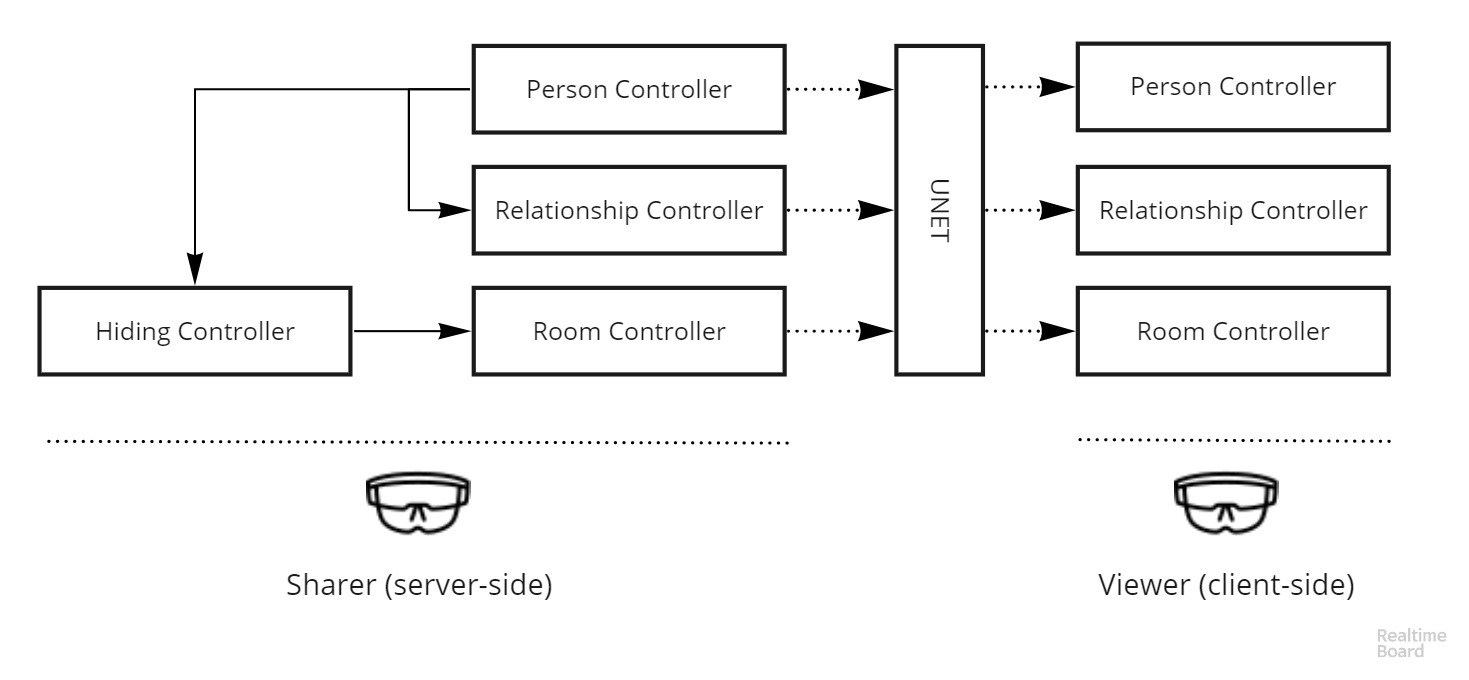
\includegraphics[width=\linewidth]{images/frontier18/system.jpg}
    \caption{The system components representing the sharer server-side (left) sharing with the viewer client-side (right) via WiFi: 1) the avatar position and orientation, 2) the social relationship data and 3) room and hidden components data. The system is built on Unity and runs on the HoloLens.}\label{fig:frontier18:system}
    \end{center}
\end{figure}

In the future, it will be possible to scan and immediately create a 3D model of the wearable AR user's surroundings. This was emulated by creating a virtual 3D room modelled to match the sharer's real room as if it had been 3D scanned.  The 3D modelling was done in Autodesk Maya\footnote{https://www.autodesk.com/education/free-software/maya} and rendered on the HoloLens display using the Unity3D\footnote{https://unity3d.com/} game engine. The avatars representing the remote people were generated using MakeHuman\footnote{http://www.makehumancommunity.org/}.

UNet\footnote{https://docs.unity3d.com/Manual/UNet.html} was used as the high-level networking API from Unity to synchronise the state of the shared room and the remote person. The state of the remote person includes 1) the position and orientation of the virtual avatar representing the remote person, and 2) the level of detail of the avatar based on the social relationship (i.e., Stranger=half 2D image, Friend=2D image, Intimate=3D avatar). The synchronised state of the room involves changing the level of detail of the shared room depending on the social relationship as well as which part of the room is hidden by the user. 

\subsection{User Study}

The prototype system explored sharing different views depending on the social relationship between users, and also different methods for maintaining privacy. A user study was conducted with 12 participants (4 female) aged (25–43, median=32, SD=4.96). Participants were asked to complete two tasks: 

Task 1: View/share a room with or without a social proximity filter (Figure \ref{fig:frontier18:social-filter}). This task had two conditions: 

\begin{figure}[H]
    \begin{center}
    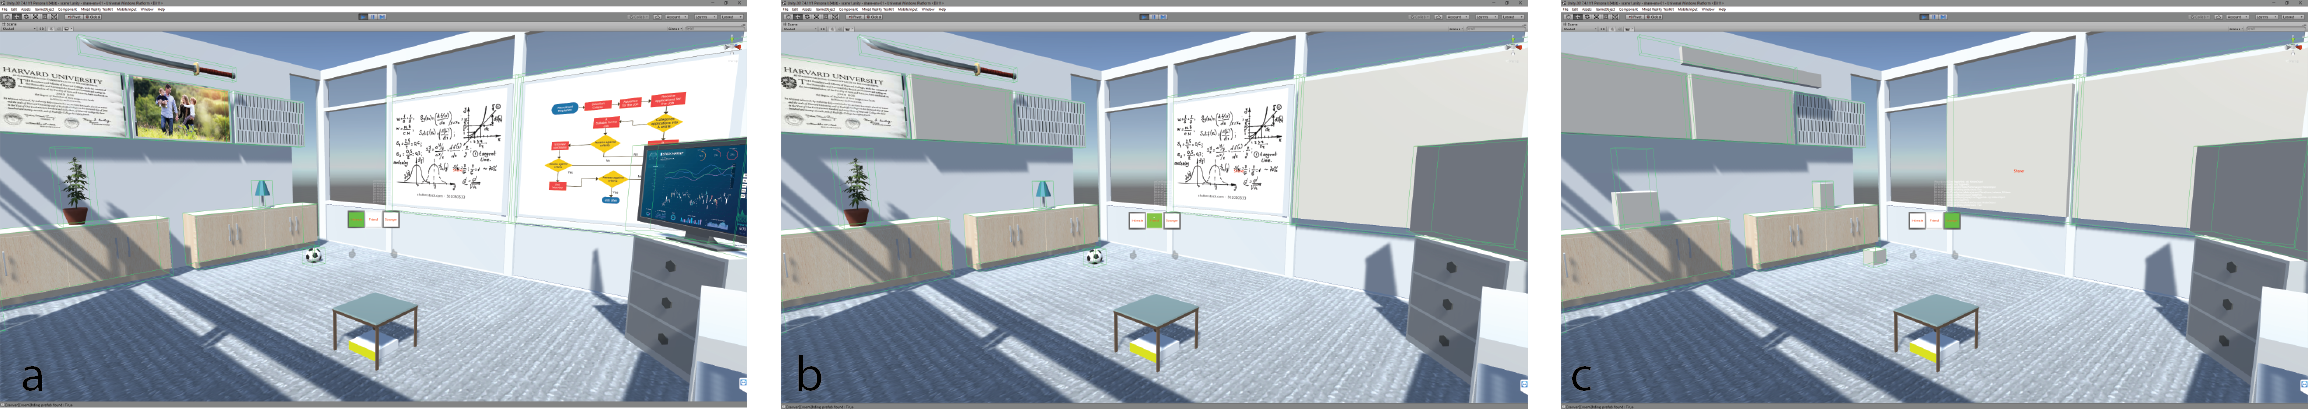
\includegraphics[width=\linewidth]{images/frontier18/images-02.png}
    \caption{A social filter applied to the shared room. a) In an Intimate relationship, everything is shared. b) For a Friend relationship, some sensitive items are hidden (e.g., family photo, stock market). c) While for a Stranger relationship almost everything is hidden in the room.}\label{fig:frontier18:social-filter}
    \end{center}
\end{figure}


\begin{itemize}
    \item T1C1: Shared room without a social proximity filter where the level of detail of the shared room is not affected by the social relationship between the users.
    \item T1C2: Shared room with a social proximity filter where the level of detail of the shared room is changed based on the social relationship between the users. 
\end{itemize}

Task 2: The mechanism of hiding/showing room parts for social proximity filter (Figure \ref{fig:frontier18:hiding-mechanism}). This task had three conditions:

\begin{itemize}
\item T2C1: Remove, where objects are hidden by being removed from the viewer's scene.
\item T2C2: Overlay, where objects are hidden by being overlaid by a white box. 
\item T2C3: Blur, where objects are hidden by appearing blurred to the viewer. 
\end{itemize}

Each participant tried the conditions from both perspectives, a viewer and a sharer. Participants were asked to rate their experience after each condition. At the end of each task, participants were asked to compare the conditions to each other and rank them. 

\begin{figure}
\begin{center}
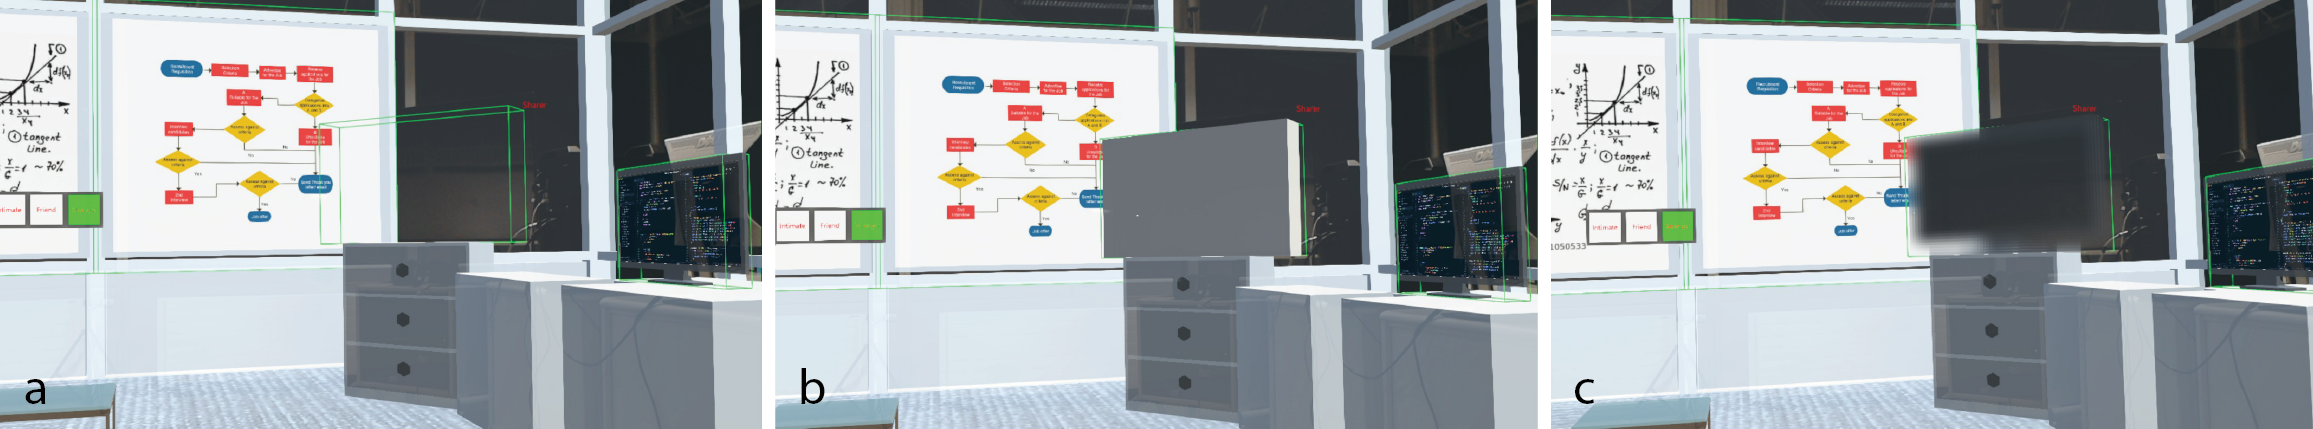
\includegraphics[width=\linewidth]{images/frontier18/images-01.png}
\caption{Hiding mechanism applied on the TV screen. a) Remove, b) Overlay, c) Blur.}\label{fig:frontier18:hiding-mechanism}
\end{center}
\end{figure}

Figure \ref{fig:frontier18:setup} shows that the experiment was set up in two similar rooms so that the sharer was sharing their room with a remote viewer. The relative position and rotation of each user were synchronised and represented as a virtual avatar in the remote person view. The sharer could change the social relationship with the viewer (Intimate, Friend, Stranger) by using 3-buttons situated in the middle of the room. The viewer could request the relationship to change by clicking on one of the relationship buttons. Once this happened, the sharer saw the relationship request in a different colour, which they then could approve and change the social relationship.

After completing each task, participants were asked to answer three sets of Likert questionnaires; six bi-polar questions (BP), six co-presence questions (CoP) and three subjective questions (S) to measure the sense of privacy (Table \ref{tab:frontier18:questions}).  

\begin{table}
    \centering
    \begin{tabular}{ll}
BP1 &    Impersonal-Personal\\
BP2 &    Cold-Warm\\
BP3 &    Colourless-Colourful\\
BP4 &    Unsociable-Sociable\\
BP5 &    Closed-Open\\
BP6 &    Passive-Active\\
CoP1    &   I noticed my partner\\
CoP2    &   My partner noticed me\\
CoP3    &   My partner's presence was obvious to me\\
CoP4    &   My presence was obvious to my partner\\
CoP5    &   My partner caught my attention \\
CoP6    &   I caught my partner's attention\\
S1  & Uncomfortable-Comfortable\\
S2  & Insecure-Secure\\
S3  & Not-Interested-Interested\\
    \end{tabular}
    \caption{The user study questionnaire included bi-polar (BP) questions, co-presence (CoP) questions and subjective (S) questions. Participants were asked to rate their experience on a 7-point Likert scale (1 = strongly disagree or negative side, 7 = strongly agree or pos)}
   side . \label{tabitive:frontier18:questions}
\end{table}

The participants were asked open-ended questions about the strengths and weaknesses of each condition. The participants were also asked to rank from most preferred to least preferred each condition for each task, then to explain the reason for why they chose the best and the worst conditions. 

\begin{figure}
\begin{center}
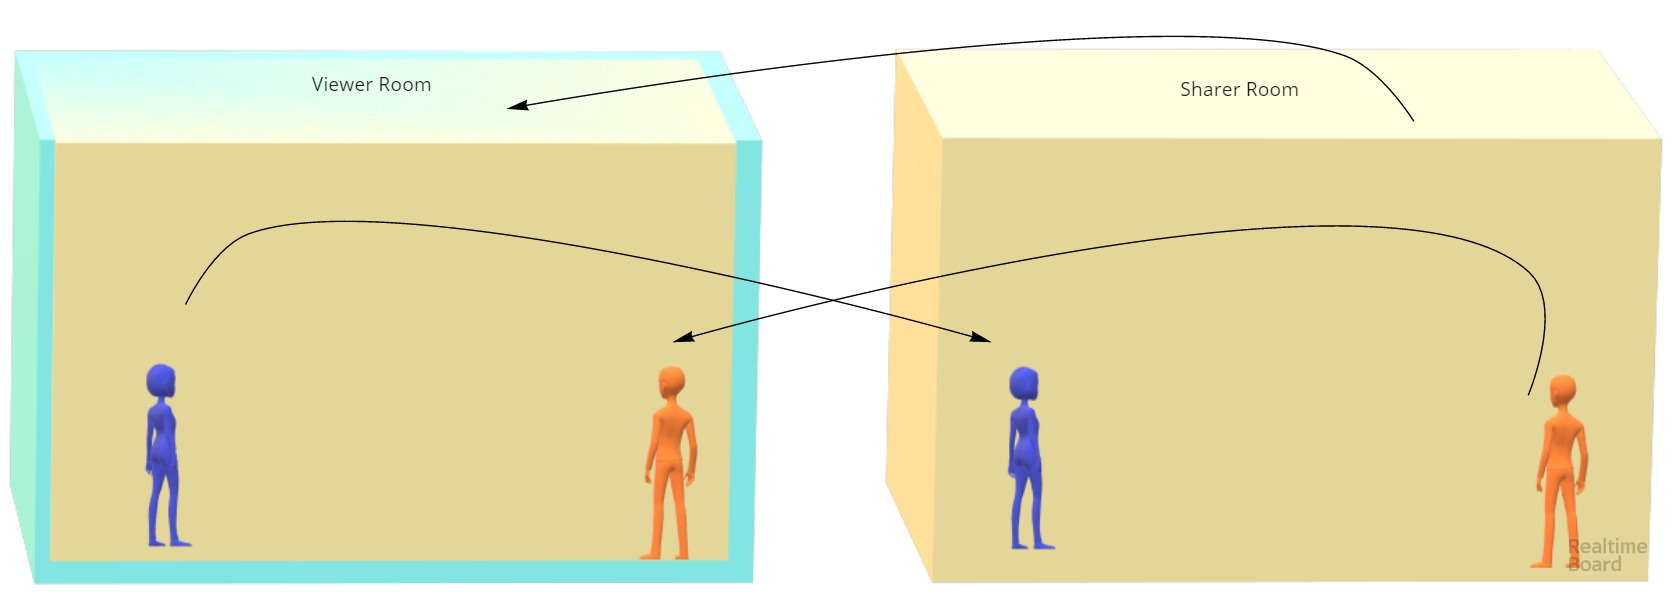
\includegraphics[width=\linewidth]{images/frontier18/experiment-setup.jpg}
\caption{The experiment setup. The sharer (right) is sharing their 3D room with the viewer (left). The viewer sees the virtual room of the sharer overlaid on top of their physical room. Each user is seeing the remote person as a virtual avatar in their environment that has the position and orientation mapped to the remote person.}\label{fig:frontier18:setup}
\end{center}
\end{figure}

\subsection{Results}

\begin{figure}
\begin{center}
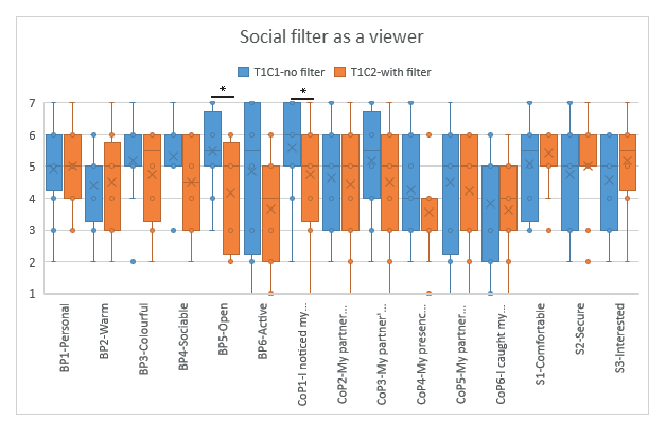
\includegraphics[width=0.8\linewidth]{images/frontier18/images-03.eps}
\caption{Results of social filter as viewer. *= statistically significant}\label{fig:frontier18:result-filter-viewer}
\end{center}
\end{figure}

\begin{figure}
\begin{center}
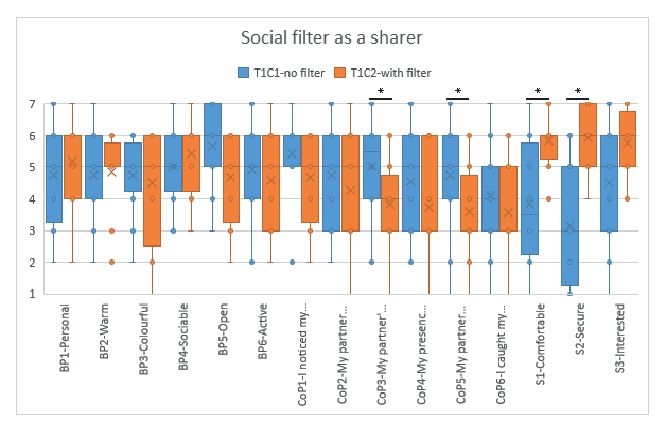
\includegraphics[width=0.8\linewidth]{images/frontier18/images-04.eps}
\caption{Results of social filter as sharer. *= statistically significant}\label{fig:frontier18:result-filter-sharer}
\end{center}
\end{figure}

Figure \ref{fig:frontier18:result-filter-viewer} shows the Likert scale results for the viewer, while Figure \ref{fig:frontier18:result-filter-sharer} shows the results for the sharer. A Wilcoxon signed-rank test on the results of Task1 comparing no social filter (T1C1) and social filter (T1C2) showed that as a viewer having a social filter (T1C2) did elicit a statistically significant difference in BP5-Open ($Z=-2.323, p=0.02$) and CoP1-I noticed my partner ($Z=-2.066, p=0.039$). While as a sharer, having a social filter (T1C2) did elicit a statistically significant difference in CoP3-My partner's presence was obvious to me ($Z=-1.993, p=0.046$) and CoP5-My partner caught my attention ($Z=-2.164, p=0.030$) and S1-Comfortable ($Z=-2.503, p=0.012$) and S2-Secure ($Z=-2.816, p=0.004$). There was no difference in response to the other questions.

\begin{figure}
\begin{center}
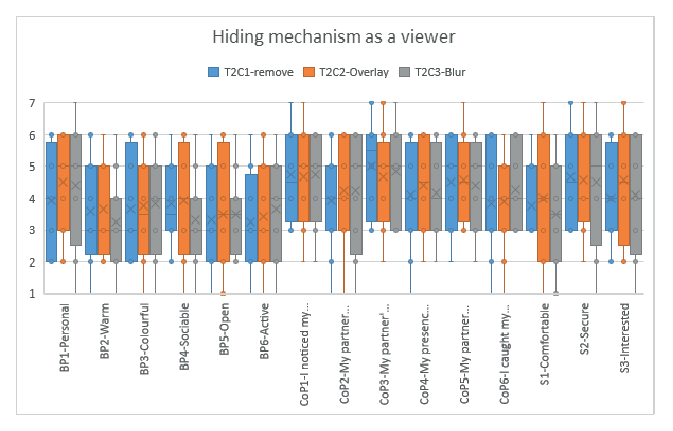
\includegraphics[width=0.9\linewidth]{images/frontier18/images-05.eps}
\caption{The results of using a hiding mechanism as a viewer.}\label{fig:frontier18:result-hiding-viewer}
\end{center}
\end{figure}

\begin{figure}
\begin{center}
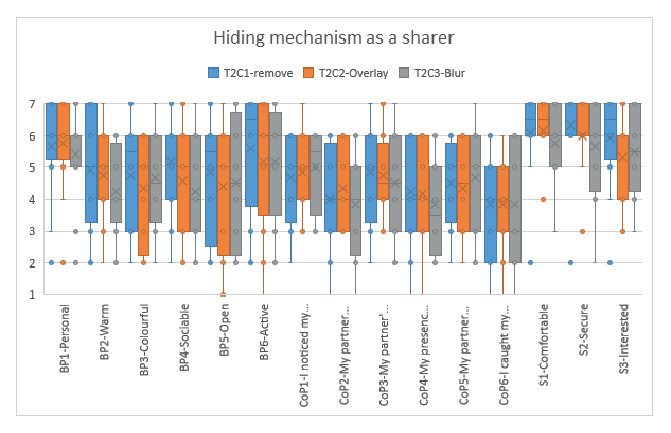
\includegraphics[width=0.9\linewidth]{images/frontier18/images-06.eps}
\caption{The results of using a hiding mechanism as a sharer.}\label{fig:frontier18:result-hiding-sharer}
\end{center}
\end{figure}

In response to the ranking questions (Figure \ref{fig:frontier18:result-ranking}), all 12 participants preferred having a social filter when sharing a view of their room over having no filter (i.e., showing everything in the room to all social relationships). As for ranking the hiding mechanism, the most preferred option for hiding sensitive data in the room was the Remove option followed by the Overlay option, while the least preferred option was Blurring. 

Participants were asked if there was a different mechanism of hiding objects in their shared room that they would prefer (such as replacing the hidden object with a similar but less sensitive one). About 42\% thought that replacing the object was a good idea; however, most of them raised concerns about how they may not like the additional effort needed for selecting a similar object to replace.

\begin{figure}
\begin{center}
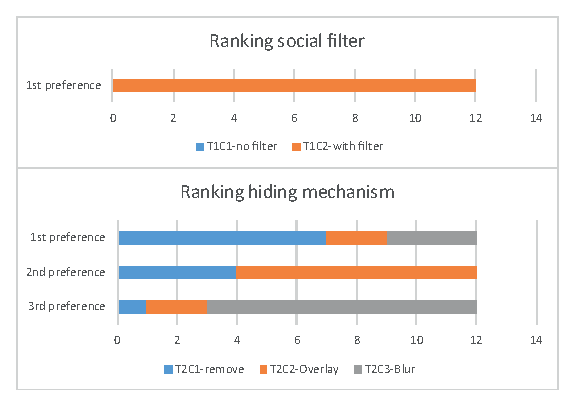
\includegraphics[width=0.8\linewidth]{images/frontier18/images-07.eps}
\caption{Results of ranking conditions.}\label{fig:frontier18:result-ranking}
\end{center}
\end{figure}

\subsection{Discussion and Future Work}

The ranking results show that having the social filter was preferred over no social filter. However, in the Likert questions, a statistical differences was found in only 2-5 questions out of 15. Participants with the sharer point of view had more statistical differences than those with the viewer point of view. This indicates that having a social filter is essential for people to feel comfortable regarding privacy when they have to choose, but not as much when they have to go through the effort of selecting which objects to hide for each social relationship.  

% In the future, we would like to allow users to customise their room so that they feel more attached to the space they are sharing. In this user study, the sharer was hiding objects in the room while the viewer was observing the shared room synchronously. In the future, we can study if hiding before the viewer is connected asynchronously would affect the sense of co-presence or the feeling of being comfortable with sharing. We would also allow participants to choose their avatars from a predefined list rather than being assigned an avatar randomly.   

\subsection{Conclusions}

This work described a HoloLens prototype built to share a 3D surrounding environment with social contacts, and simulate a future wearable AR social networking application. The prototype was designed to explore how users would be willing to share views of their surroundings with remote people with different social relationships. 

Participants were allowed to choose which part of the room to hide or show to different social groups (Intimate, Friend, Stranger). A user study was run to test the effects of using a social filter on co-presence and feelings of privacy from both sides, as a sharer and a viewer. Results showed that all participants preferred having a social filter, and that there was some statistical difference regarding feelings of co-presence and privacy. 

